\documentclass[handout]{beamer}

\title{Nuclear penalized multinomial regression}
\author{\color{ricerichblue} Scott Powers \\ \color{ricegray} \scriptsize (Joint work with Trevor Hastie and Rob Tibshirani)}
\date{Rice Statistics Colloquium \\ April 17, 2023}

\usepackage{hyperref, mathrsfs, tabto, tikz, ulem}
\usecolortheme[RGB={0, 32, 91}]{structure}  % Rice blue
\usetheme{Singapore}
\setbeamertemplate{navigation symbols}{\insertframenumber}

\definecolor{dodgerblue}{rgb}{0.12, 0.56, 1.0}
\definecolor{darkorange}{rgb}{1.0, 0.55, 0.0}
\definecolor{forestgreen}{rgb}{0.13, 0.55, 0.13}
\definecolor{riceblue}{rgb}{0.000, 0.125, 0.357}
\definecolor{ricegray}{rgb}{0.486, 0.494, 0.498}
\definecolor{ricerichblue}{rgb}{0.039, 0.314, 0.620}

\def\A{\mathcal A}\def\B{\mathcal B}\def\C{\mathcal C}\def\D{\mathcal D}
\def\E{\mathcal E}\def\F{\mathcal F}\def\G{\mathcal G}\def\J{\mathcal J}
\def\K{\mathcal K}
\def\L{\mathcal L}\def\M{\mathcal M}\def\N{\mathcal N}\def\O{\mathcal O}
\def\P{\mathcal P}\def\Q{\mathcal Q}\def\R{\mathcal R}\def\S{\mathcal S}
\def\T{\mathcal T}\def\W{\mathcal W}\def\V{\mathcal V}\def\X{\mathcal X}
\def\Y{\mathcal Y}\def\Z{\mathcal Z}
\def\mE{\mathbb E}\def\mI{\mathbb I}\def\mN{\mathbb N}\def\mP{\mathbb P}
\def\mR{\mathbb R}\def\mS{\mathbb S}
\def\bA{{\bf A}}\def\bB{{\bf B}}\def\bC{{\bf C}}\def\bE{{\bf E}}\def\bP{{\bf P}}
\def\bU{{\bf U}}\def\bV{{\bf V}}\def\bX{{\bf X}}\def\bY{{\bf Y}}
\def\bb{{\bf b}}\def\bu{{\bf u}}\def\bv{{\bf v}}\def\bx{{\bf x}}
\def\balpha{{\bf \alpha}}\def\bSigma{{\bf \Sigma}}
\def\HR{{\mbox{\scriptsize HR}}}
\def\prob{\mbox{\bf prob}}\def\tr{\mbox{\bf tr}}
\def\l{\left}\def\r{\right}\def\lf{\lfloor}\def\rf{\rfloor}
\def\un{\underline}
\def\theat{\theta}\def\lambad{\lambda}\def\lamda{\lambda}
\def\iid{\stackrel{\mbox{\scriptsize i.i.d.}}{\sim}}
\def\ind{\stackrel{\mbox{\scriptsize ind.}}{\sim}}
\def\minimize{\mbox{minimize}\hspace{4mm}}
\def\maximize{\mbox{maximize}\hspace{4mm}}
\def\subjectto{\mbox{subject to}\hspace{4mm}}
\newcommand\bovermat[3]{\makebox[0pt][l]{$\smash{\overbrace{\phantom{
      \begin{matrix}#3\end{matrix}}}^{\text{#1}}}$}#2}

\begin{document}

\begin{frame}
  \maketitle
  \vfill
  \hfill
  \includegraphics[width = 0.5\textwidth]{images/rice_smgt.png}
\end{frame}

\begin{frame}{Background}
  \begin{columns}
    \begin{column}{0.4\textwidth}
      \includegraphics[width = \textwidth]{images/bases.png}
    \end{column}
    \begin{column}{0.6\textwidth}
      \begin{itemize}
        \item Game is a sequence of matchups between one pitcher and one batter
        \item Batters try to advance along bases before recording 3 outs
        \item Markov chain model works well
        \begin{itemize}
          \item State space: \{bases, outs\}
        \end{itemize}
      \end{itemize}
    \end{column}
  \end{columns}
  \vspace{4mm}
  \pause
  (Essentially) 9 possible outcomes of each batter-pitcher matchup:
  \begin{center}
    \small
    \begin{tabular}{ccccccccc}
       \color{ricerichblue} HR    & \color{ricerichblue} 3B    & \color{ricerichblue} 2B    & \color{ricerichblue} 1B    & \color{ricerichblue} HBP   & \color{ricerichblue} BB    & \color{ricegray} K     & \color{ricegray} G     & \color{ricegray} F\\
       \color{ricerichblue}  1.38 & \color{ricerichblue}  1.06 & \color{ricerichblue}  0.76 & \color{ricerichblue}  0.46 & \color{ricerichblue}  0.35 & \color{ricerichblue}  0.33 & \color{ricegray} -0.27 & \color{ricegray} -0.27 & \color{ricegray} -0.27
     \end{tabular}
  \end{center}
\end{frame}

\begin{frame}{Predicting player performance}
  Baseball analysis blogs (early 2010s):
  \begin{itemize}
    \item ``Stabilization rate'':\\
      Sample size at which between-sample correlation is 0.7
    \begin{itemize}
      \item wOBA: $n = 350$
      \item K\%: $n = 60$
      \item BABIP: $n = 1200$
    \end{itemize}
    $$
      \mbox{BABIP} = \frac
        {\mbox{1B} + \mbox{2B} + \mbox{3B}}
        {\mbox{1B} + \mbox{2B} + \mbox{3B} + \mbox{G} + \mbox{F}}
    $$
  \end{itemize}
  ~\\
  \pause
  Powers and Shayer (SABR Analytics 2016):
  \begin{itemize}
    \item Multinomial regression with ridge penalty
    \begin{itemize}
      \item Two categorical variables (batter and pitcher), plus controls
      \item Adjusts player performance for competition and sample size
      \item Similar to random-effect models and Bayesian models
    \end{itemize}
  \end{itemize}
\end{frame}

\begin{frame}{Notation}
  \begin{itemize}
    \item $i = 1, ..., n$, indexes plate appearances (PA)
    \item Within the $i^{th}$ PA, ...
    \begin{itemize}
      \item Batter $B_i \in \B = \mbox{\{Mike Trout, ..., Zach Cozart\}}$
      \item Pitcher $P_i \in \P = \mbox{\{Clayton Kershaw, ..., Zack Britton\}}$
      \item Outcome $y_i \in \O = \mbox{\{F, G, K, BB, HBP, 1B, 2B, 3B, HR\}}$
    \end{itemize}
  \end{itemize}
  ~\\
  Model:
  $$\mP(Y_i = k) = \frac{e^{\eta_{ik}}}{\sum_{k' \in \O}e^{\eta_{ik'}}}$$
  $$\eta_{ik} = \alpha_k + \beta_{k:B_i} + \gamma_{k:P_i}$$
  ~\\
  Objective:
  $$\underset{\alpha, \beta, \gamma}{\mbox{minimize}}
    -\sum_{i=1}^n\log\mP(Y_i = y_i) + \lambda\sum_{k \in \O}
    \l(\sum_{B \in \B}\beta_{k:B}^2 + \sum_{P \in \P}\gamma_{k:P}^2\r)$$
\end{frame}

\begin{frame}{Matrix notation}
\scriptsize
$$\bX = \l(\begin{array}{llllll}
        \bovermat{Batters}{1&...&0}{...&...&...}&
        \bovermat{Pitchers}{0&...&0}{...&...&...}\\
        0&...&0&0&...&1\\
        0&...&0&1&...&0\\
        ...&...&...&...&...&...\\
        0&...&1&0&...&0\\
        0&...&0&0&...&0
    \end{array}\r)
\hspace{1cm}
\bB = \l(\begin{array}{lll}
  \beta_{F:MT}&...&\beta_{HR:MT}\\
  ..&...&..\\
  \beta_{F:ZC}&...&\beta_{HR:ZC}\\
  \gamma_{F:CK}&...&\gamma_{HR:CK}\\
  ..&...&..\\
  \gamma_{F:ZB}&...&\gamma_{HR:ZB}
\end{array}\r)$$
    $$\hspace{10mm} \underbrace{n\times(|\B|+|\P|)}_{n \times p}
    \hspace{35mm} \underbrace{(|\B| + |\P|)\times|\O|}_{p\times K}$$
  \vspace{4mm}
    \normalsize 
$$\underset{\balpha\in\mR^K,~\bB\in\mR^{p\times K}}{\mbox{minimize}}
  -\underbrace{\sum_{i=1}^n\log\l(\sum_{k=1}^K\frac{e^{\alpha_k + \bX\bb_k}}
  {\sum_{k' = 1}^Ke^{\alpha_{k'} + \bX\bb_{k'}}}\mI_{\{y_i = k\}}\r)}_{
  \normalsize =~\ell(\alpha, \bB; \bX, \bY)}
  + \lambda||\bB||_F^2$$
  \pause
  \begin{itemize}
    \item \# parameters: \hspace{4mm} $K + p \times K = 9 + 764 \times 9 = 6885$
  \end{itemize}
\end{frame}

\begin{frame}{Structure between plate appearance outcomes}
Ordering:
$$\mbox{K $<$ G $<$ F $<$ BB $<$ HBP $<$ 1B $<$ 2B $<$ 3B $<$ HR}$$
\pause
Structure:
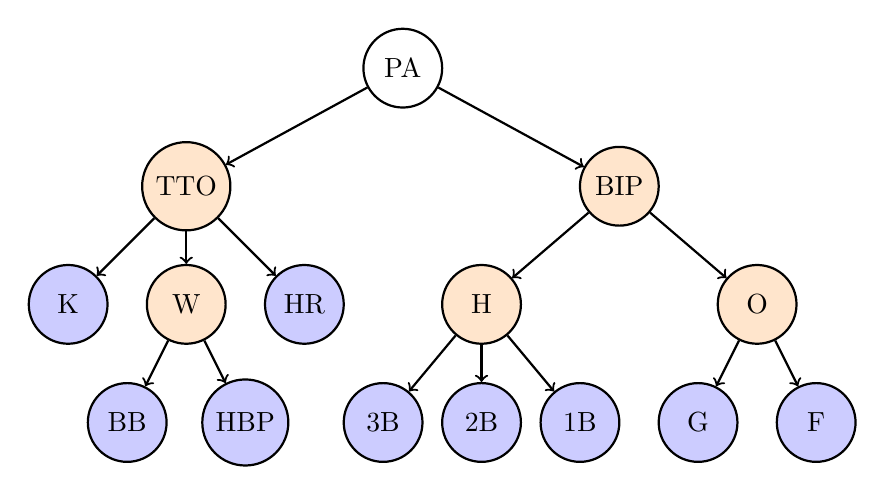
\begin{tikzpicture}[->,thick,
    leaf/.style={circle,draw,minimum size=1cm,fill=blue!20},
    split/.style={circle,draw,minimum size=1cm,fill=orange!20},
    head/.style={circle,draw,minimum size=1cm}]
\node[leaf] (BB) at (0, 0) {BB};
\node[leaf] (HBP) at (1.5, 0) {HBP};
\node[leaf] (3B) at (3.25, 0) {3B};
\node[leaf] (2B) at (4.5, 0) {2B};
\node[leaf] (1B) at (5.75, 0) {1B};
\node[leaf] (G) at (7.25, 0) {G};
\node[leaf] (F) at (8.75, 0) {F};
\node[leaf] (K) at (-0.75, 1.5) {K};
\node[split] (W) at (0.75, 1.5) {W};
\node[leaf] (HR) at (2.25, 1.5) {HR};
\node[split] (H) at (4.5, 1.5) {H};
\node[split] (O) at (8, 1.5) {O};
\node[split] (TTO) at (0.75, 3) {TTO};
\node[split] (BIP) at (6.25, 3) {BIP};
\node[head] (PA) at (3.5, 4.5) {PA};
\path
    (PA) edge (TTO)
    (PA) edge (BIP)
    (TTO) edge (K)
    (TTO) edge (W)
    (TTO) edge (HR)
    (BIP) edge (H)
    (BIP) edge (O)
    (W) edge (BB)
    (W) edge (HBP)
    (H) edge (3B)
    (H) edge (2B)
    (H) edge (1B)
    (O) edge (G)
    (O) edge (F);
\end{tikzpicture}\\
\hfill{\tiny \color{gray} Adapted from Baumer \& Zimbalist (2014)}
\end{frame}

\begin{frame}{Principal component analysis of observed rates}
  Batters:
  \begin{center}
    \includegraphics[width = .8\textwidth]{figures/pca_bat_fancy.pdf}\\
  \end{center}
  Pitchers:
  \begin{center}
    \includegraphics[width = .8\textwidth]{figures/pca_pit_fancy.pdf}
  \end{center}
\end{frame}

\begin{frame}{Reduced-rank multinomial regression}
  \begin{align*}
    \underset{\balpha\in\mR^K,~\bB\in\mR^{p\times K}}{\mbox{minimize}} &
      -\ell(\alpha, \bB; \bX, \bY)\\
    \mbox{subject to} &
      \hspace{5mm}\mbox{rank}(\bB) \le r\\
    \\
    &
      \color{ricerichblue} \Rightarrow \exists~\bA\in\mR^{p\times r}, \bC\in\mR^{K\times r} \mbox{ s.t. } \bB = \bA\bC^T
  \end{align*}
  \begin{itemize}
    \item CRAN package {\tt VGAM} implements reduced-rank vector generalized linear
      models (RR-VGLMs, Yee and Hastie, 2003)
    \item Far too slow to fit on full season of MLB play-by-play data
    \begin{itemize}
      \item Not a convex optimization problem
    \end{itemize}
  \end{itemize}
\end{frame}

\begin{frame}{Nuclear penalized multinomial regression}
NPMR:
$$\underset{\balpha\in\mR^K,~\bB\in\mR^{p\times K}}{\mbox{minimize}}
  - \ell(\alpha, \bB; \bX, \bY) + \lambda||\bB||_*$$
\vspace{5mm}
$$||\bB||_* = \sum_{r=1}^{\mbox{\scriptsize rk}(\bB)}\sigma_r$$
\begin{itemize}
\item Convex relaxation of reduced-rank regression\\
  \small \color{ricegray} (Just as the lasso is a convex relaxation of best subset regression!)
%\item Solved via {\bf accelerated} proximal gradient descent
%\item Implemented on CRAN in {\tt npmr}
\end{itemize}
\end{frame}

\begin{frame}{How to solve it?}
  $$
    \underset{\bB\in\mR^{p\times K}}{\mbox{minimize}}
      -\ell(\bB; \bX, \bY) + \lambda||\bB||_*
  $$
  \begin{enumerate}
    \pause
    \item Alternating direction method of multipliers (ADMM)\\
      ~\\
      Variable splitting:
      \begin{align*}
        \underset{\bB,\bC\in\mR^{p\times K}}{\mbox{minimize}} &
          -\ell(\bB; \bX, \bY) + \lambda||\bC||_*\\
        \mbox{subject to} & \hspace{2mm} \bB - \bC = 0
      \end{align*}
    \pause
    \item Proximal gradient descent (PGD)
  \end{enumerate}
\end{frame}

\begin{frame}{Proximal gradient descent}
  \begin{itemize}
    \item Gradient descent:
      \small
      \begin{align*}
        \hspace{-1cm}
        \bB^{(t+1)} &= \bB^{(t)} - s\nabla {\color{ricerichblue} f}(\bB^{(t)})\\
                    &= \underset{\bB \in \mathbb{R}^{p \times K}}{\arg\min}\left\{
                      {\color{ricerichblue} f}(\bB^{(t)}) +
                        \left\langle
                          \nabla {\color{ricerichblue} f}(\bB^{(t)}),
                          \bB - \bB^{(t)}
                        \right\rangle +
                        \frac{1}{2s}||\bB - \bB^{(t)}||_F^2
                    \right\}
      \end{align*}
      \normalsize
    \pause
    \item {\bf Proximal} gradient descent (PGD)
      \small
      \begin{align*}
        \hspace{-1cm}
        \bB^{(t+1)} &= \underset{\bB \in \mathbb{R}^{p \times K}}{\arg\min}\left\{
                      {\color{ricerichblue} g}(\bB^{(t)}) +
                        \left\langle
                          \nabla {\color{ricerichblue} g}(\bB^{(t)}),
                          \bB - \bB^{(t)}
                        \right\rangle +
                        \frac{1}{2s}||\bB - \bB^{(t)}||_F^2 +
                        {\color{ricerichblue} h}(\bB)
                    \right\}\\
                    &{\color{ricegray}
                      \mbox{Proximal operator: }
                      {\bf prox}_{h}(z) \equiv \arg\min_\theta\left\{
                        \frac12||z - \theta||_2^2 + h(\theta)
                      \right\}
                    }\\
                    &= {\bf prox}_{s\color{ricerichblue}h}\left(
                      \bB^{(t)} - s\nabla {\color{ricerichblue} g}(\bB^{(t)})
                    \right)
      \end{align*}
      \normalsize
  \end{itemize}
\end{frame}

\begin{frame}{Proximal gradient descent}
Proximal map for nuclear norm: soft-thresholding singular values
$$\bB = \bU\bSigma\bV^T \hspace{1cm} [\mathcal S_{s\lambda}(\bSigma)]_{rr} =
    (\sigma_r - s\lambda)_+$$
$${\bf prox}_{s\lambda||\cdot||_*}(\bB) =
    \bU{\mathcal S_{s\lambda}(\bSigma)}\bV^T$$
\vspace{4mm}\\
\pause
Repeat until convergence:
\begin{enumerate}
    \item $\alpha^{(t+1)} = \alpha^{(t)} + s{\bf1}^T\l(\bY -
      \hat\bP(\alpha^{(t)}, \bB^{(t)})\r)$
    \item $\bB^{(t+1)} = {\bf prox}_{s\lambda||\cdot||_*}\l(\bB^{(t)} +
      s\bX^T\l(\bY - \hat\bP(\alpha^{(t)}, \bB^{(t)})\r)\r)$
\end{enumerate}
\vspace{4mm}
sublinear convergence (Nesterov, 2007) b/c $\nabla\ell$ is Lipschitz
\end{frame}

\begin{frame}{Accelerated PGD}
Initialize $\alpha^{(0)}, \bA^{(0)}, \bB^{(0)}$, and iterate until convergence:
\begin{enumerate}
    \item $\alpha^{(t+1)} = \alpha^{(t)} +
      s{\bf1}^T\l(\bY - \hat\bP(\alpha^{(t)}, \bA^{(t)})\r)$
    \item {\color{ricerichblue} $\bA^{(t+1)} = \bB^{(t)} + \frac t{t+3}(\bB^{(t)} - \bB^{(t-1)})$}
    \item $\bB^{(t+1)} = {\bf prox}_{s\lambda||\cdot||_*}\l(\bA^{(t+1)} +
      s\bX^T\l(\bY - \hat\bP(\alpha^{(t+1)}, \bA^{(t+1)})\r)\r)$
\end{enumerate}
\vspace{4mm}
{\bf Much} faster! Implemented on CRAN in {\tt npmr} package.
\end{frame}

\begin{frame}{Simulation study}
  $Y_i$ simulated independently from:
  $$\mP(Y_i = k) = \frac{e^{\bX\beta_k}}
      {\sum_{\ell=1}^8e^{\bX\beta_\ell}}\mbox{ for }i = 1, ..., n\mbox{ and }
      k = 1, ..., 8$$
  $$\bx_i \iid \mbox{Normal}(\vec 0_{12}, \mI_{12})$$
  \begin{columns}
    \begin{column}{.5\textwidth}
      \centering
      {\bf Full rank setting}
      $$B_{jk} \iid \mbox{Normal}(0, 1)$$
      $$~$$
      $$~$$
    \end{column}
    \begin{column}{.5\textwidth}
      \centering
      {\bf Low rank setting}
      $$\bB_{12\times8} = \bA_{12\times2}\bC_{2\times8}$$
      $$A_{j\ell} \iid \mbox{Normal}(0, 1)$$
      $$C_{\ell k} \iid \mbox{Normal}(0, 1)$$
    \end{column}
  \end{columns}
\end{frame}

\begin{frame}{Simulation results}
\includegraphics[width = .5\textwidth]{figures/sim_full.pdf}\hfill
\includegraphics[width = .5\textwidth]{figures/sim_low.pdf}
\end{frame}

\begin{frame}{Baseball application details}
\begin{itemize}
\item $n =$ 181,577 PA. For $i^{th}$ PA, observe:
    \begin{itemize}
    \item $B_i$: {\bf B}atter (403 unique batters)
    \item $P_i$: {\bf P}itcher (361 unique pitchers)
    \item $S_i$: {\bf S}tadium
    \item $H_i$: indicator batter is on {\bf H}ome team
    \item $O_i$: indicator batter has {\bf O}pposite handedness of pitcher's
    \end{itemize}
\end{itemize}
Model:
$$\mP(Y_i = k) = \frac{e^{\eta_{ik}}}{\sum_{k' \in \O}e^{\eta_{ik'}}}
    \mbox{for $k \in \O$, where}$$
$$\eta_{ik} = \alpha_k + \beta_{k:B_i} + \gamma_{k:P_i} + \delta_{k:S_i} +
    \zeta_kH_i + \theta_kO_i$$
Objective:
$$\underset{\balpha\in\mR^9,~\bB\in\mR^{796\times 9}}{\mbox{minimize}}
  -\ell(\alpha,\bB;\bX,\bY) + \lambda(||\bB_\B||_*+||\bB_\P||_*+||\bB_\S||_*)$$
\end{frame}

\begin{frame}{Results}
Batters:
\begin{center}
\includegraphics[width = .8\textwidth]{figures/B_bat_fancy.pdf}\\
\end{center}
Pitchers:
\begin{center}
\includegraphics[width = .8\textwidth]{figures/B_pit_fancy.pdf}
\end{center}
\end{frame}

\begin{frame}{Results}
\tiny
\hspace{-4mm}
\begin{tabular}{c}
\\\\
{\bf Tool}\\
\\\\
{\bf Top}\\
{\bf 5}\\
\\\\\\\\
{\bf Bot}\\
{\bf 5}\\
\\\\\\
\end{tabular}
\begin{tabular}{|c|c|c|c|}
\multicolumn{3}{c}{\bf\normalsize Batters}\\
\multicolumn{3}{c}{}\\
\hline
{\bf Patience}  & {\bf Trajectory}  & {\bf Speed}\\
\hline
\hline
More K, BB      & More F            & More 1B\\
\hline
P Bourjos       & I Kinsler         & Y Cespedes\\
E Rosario       & F Freeman         & L Cain\\
C Santana       & O Infante         & J Iglesias\\
G Springer      & K Wong            & K Kiermaier\\
M Napoli        & J Altuve          & D DeShields Jr\\
                &                   &\\
J Reddick       & D Gordon          & E Longoria\\
JT Realmuto     & A Rodriguez       & R Howard\\
AJ Pollock      & C Maybin          & O Herrera\\
K Pillar        & S Choo            & S Smith\\
E Aybar         & F Cervelli        & J Lamb\\
\hline
More F, G, 1B   & More G, 1B        & More G\\
\hline
\end{tabular}
\hfill
\begin{tabular}{|c|c|c|c|c|}
\multicolumn{3}{c}{\bf\normalsize Pitchers}\\
\multicolumn{3}{c}{}\\
\hline
{\bf Power} & {\bf Trajectory}  & {\bf Command}\\
\hline
\hline
More K      & More F            & More F, G, K\\
\hline
J Quintana  & J Chavez          & M Scherzer\\
C Kluber    & J Verlander       & M Tanaka\\
M Bumgarner & J Peavy           & J deGrom\\
M Scherzer  & J Cueto           & R de la Rosa\\
C Kershaw   & C Young           & M Harvey\\
            &                   &\\
J Danks     & D Keuchel         & M Pelfrey\\
D Haren     & G Richards        & C Tillman\\
C Hamels    & S Dyson           & E Butler\\
A Sim\'{o}n & B Anderson        & G Gonzalez\\
RA Dickey   & M Pineda          & J Samardzija\\
\hline
More F, G   & More G            & More BB, 1B\\
\hline
\end{tabular}
\end{frame}

\begin{frame}{Validation of NPMR v ridge regression}
\centering
\includegraphics[width = 0.8\textwidth]{figures/baseball_test.pdf}
\end{frame}

\begin{frame}{Vowel data set}
Robinson (1989) vowel data:
\begin{center}
\begin{tabular}{cc|cc}
Vowel   & Word  & Vowel & Word\\
\hline
i       & heed  & O     & hod\\
I       & hid   & C:    & hoard\\
E       & head  & U     & hood\\
A       & had   & u:    & who'd\\
a:      & hard  & 3:    & heard\\
Y       & hud
\end{tabular}
\end{center}
\begin{itemize}
    \item 15 subjects (8 in training set, 7 in test set)
    \item $K = 11$, $n = 528$, $p = 10$ and $m = 462$
\end{itemize}
\end{frame}

\begin{frame}{Results on vowel data}
\centering
\includegraphics[width = 0.8\textwidth]{figures/vowel.pdf}
\end{frame}

\begin{frame}{Results on vowel data}
\centering
\includegraphics[width = \textwidth]{figures/B_vowel_fancy.pdf}\\
\end{frame}

\begin{frame}{Back to baseball: Better data}
  \centering
  \includegraphics[width = 0.7\textwidth]{figures/xwoba.pdf}
  \begin{itemize}
    \item In addition to outcome, we observe batted ball characteristics: exit velocity, launch angle, bearing
    \item Powers (Saberseminar 2016): Model the joint distribution of exit velocity and launch angle by batter-pitcher matchup
  \end{itemize}
\end{frame}

\begin{frame}{Lessons learned from 6 seasons in baseball}
  \begin{enumerate}
    \item Start simple! Start with the data\\~\\
    \item Edge cases {\it really} matter\\~\\
    \item Recommended reading:\\~\\
      \centering
      \includegraphics[height = 1in]{images/thinking_fast_and_slow.jpg}
      \hspace{1cm}
      \includegraphics[height = 1in]{images/escape_from_model_land.jpg}
  \end{enumerate}
\end{frame}

\begin{frame}{Upcoming projects}
  \begin{itemize}
    \item Predicting future outcomes from pitch trajectories
    \item Swing biomechanics
    \item Volleyball analytics
  \end{itemize}
\end{frame}

\begin{frame}{Predicting future outcomes from pitch trajectories}
  \centering
  \includegraphics[width = 0.7\textwidth]{images/pitch_tracking.png}
  \begin{itemize}
    \item {\bf Data:} Each pitch generates $\vec X \in \mR^9$ estimating flight path as a 3-dimensional quadratic in time
    \item {\bf Problem:} Predict a pitcher's {\it future} results based on tracking data from past pitches thrown
  \end{itemize}
\end{frame}

\begin{frame}{Swing biomechanics}
  \begin{columns}
    \begin{column}{0.4\textwidth}
      \includegraphics[width = \textwidth]{images/swing_biomechanics.jpeg}
    \end{column}
    \begin{column}{0.6\textwidth}
      \begin{itemize}
        \item {\bf Data:} Each swing generates time series $\{\vec Y_t\} \in \mR^{56}$ for $t = 1, ..., 300$
        \item {\bf Problem:} Develop a statistic to measure swing adaptability
      \end{itemize}
    \end{column}
  \end{columns}
\end{frame}

\begin{frame}{Volleyball analytics}
  \centering
  \includegraphics[width = 0.7\textwidth]{images/volleyball.png}
  \begin{itemize}
    \item {\bf Data:} Manually charted touch-by-touch data for over a decade of NCAA women's Division I volleyball
    \item {\bf Problem:} What is the magnitude of the effect that individual actions have on team performance?
  \end{itemize}
\end{frame}

\begin{frame}
\centering
\Large
Thank You!
\end{frame}

\begin{frame}{References}
\footnotesize
Anderson (1984) Regression and ordered categorical variables. {\it JRSS B}\\~\\
Baumer and Zimbalist (2014) {\it The Sabermetric Revolution}\\~\\
Hastie, Tibshirani and Wainwright (2015) {\it Statistical Learning with
    Sparsity: The Lasso and Generalizations}\\~\\
Lu et al. (2009) Convex optimization methods for dimension reduction and
    coefficient estimation in multivariate linear regression.
    {\it Mathematical programming}\\~\\
Toh and Yun (2009) An accelerated proximal gradient algorithm for nuclear norm
    regularized linear least squares problems.
    {\it Pacific Journal of Optimization}\\~\\
Yee and Hastie (2003) Reduced-rank vector generalized linear models.
    {\it Statistical Modelling}\\~\\
Yuan et al. (2007) Dimension reduction and coefficient estimation in
multivariate linear regression. {\it JRSS B}
\end{frame}

\end{document}
